\documentclass{beamer}

% \usepackage{beamerthemesplit} // Activate for custom appearance

\usepackage[english]{babel}
\usepackage[utf8x]{inputenc}
\usepackage{amsmath}
\usepackage{graphicx}

\title{7.0 Limits and derivatives (12.1 IB SL)}
\author{Dr. Huson}
\date{\today}

\begin{document}

\frame{\titlepage}

\section[Outline]{}
\frame{\tableofcontents}

\section{Drui}
\frame
{
  \frametitle{How do we use limits?}

  \begin{itemize}
  \item CCSS: Limits
  \item Do Now: Prior learning problems
  \item Lesson: Introduction to limits     
  \item Homework:     
  \end{itemize}
}

\section{Prior learning}
\frame
{
  \frametitle{Prior learning}

  \begin{itemize}
  \item Factoring polynomials
  \item Expanding powers of binomials
  \item Rational exponents     
  \end{itemize}
}
%This slide should be set up by the paper cutting investigation on page 196.
%Students should put data table and graph on the board.
\section{Limits of sequences}
\frame
{
  \frametitle{Limits of sequences}
  \only<1>{Consider this sequence. If it went on forever, what would it's value be?}
  \only<2>{Notation: \[\lim_{n \rightarrow \infty} {u_n} = L\]}
  \only<2>{"The limit as \emph{n} approaches infinity of \emph{u} sub \emph{n} equals \emph{L}."}
{\renewcommand{\arraystretch}{1.25}
\begin{table}
\centering
\begin{tabular}{l|r}
Element & Value \\\hline
$u_1$ & $\frac {1}{3}$ \\
$u_2$ & $\frac {4}{9}$ \\
$u_3$ & $\frac {13}{27}$ \\
$u_4$ & $\frac {40}{81}$ \\
$\vdots$ & $\vdots$
\end{tabular}
\end{table}
}}

\section{Convergence and divergence}
\frame
{
  \frametitle{Convergence and divergence}
\begin{definition}
A \alert{Convergent} sequence approaches a fixed value (real number).\\
Example: $\frac {1}{3}, \frac {4}{9}, \frac {13}{27},  \frac {40}{81}, \dots$ (approaches $\frac {1}{2}$)\\[5pt]
A \alert{Divergent} sequence does not converge.\\
Example: 1, 1, 2, 3, 5, 8, 13, $\dots$
\end{definition}
\begin{flushright}
    Example 1 page 197\\
    Exercise 7A
\end{flushright}
}

\section{Limit of a function}
\frame
{
  \frametitle{Limit of a function}
  \begin{definition}
  A function, $f(x)$, is said to have a \alert{limit} for a specific input value, $c$, if as $x$ gets sufficiently close to $c$ (from either side), $f(x)$ gets close to a value, $L$.\\
Notation: \[\lim_{x \rightarrow c} {f(x)} = L\]
  \end{definition}
}

\section{Limit of a function}
\subsection{Examples}
\frame
{
  \frametitle{Limit of a function}
\begin{example}
Find the limit or state that it does not exist.
\begin{enumerate}[(a)]
\item $\displaystyle{\lim_{x \rightarrow 2}{x^2}}$\\
\item $\displaystyle{\lim_{x \rightarrow 1}{\frac{x^2-1}{x-1}}}$
\item $\displaystyle{\lim_{x \rightarrow 0}{f(x)}} \text{ where } f(x)= \left \{
\begin{array}{rl}
1 & \text{ for } x\geq 0 \\ 
-1 & \text{ for } x\leq 0 
\end{array}
\right.$
\end{enumerate}
\end{example}
}

\section{Limit of a function}
\subsection{Example (b)}
\frame
{
  \frametitle{Limit of a function}
\only<1>{Example 2(b) pg. 198 \\
Find the limit or state that it does not exist.}
\[\displaystyle{\lim_{x \rightarrow 1}{\frac{x^2-1}{x-1}}}\]
\only<1>{Three approaches: graphing, algebra, data table}
\only<2>{
Graphing:
\begin{figure}
    \centering
    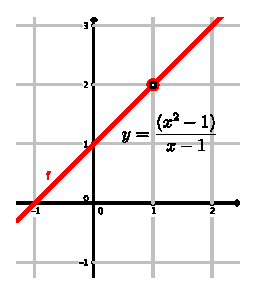
\includegraphics{Ex2b-pg199-graph.eps}
\end{figure}
Note the \alert{discontinuity}.}
\only<3>{
Algebra:
\[f(x) = {\frac{x^2-1}{x-1}} 
= {\frac{(x+1)(x-1)}{x-1}} = x+1 \]
\flushright{\alert{$x \neq 1$}}}
\only<4>{
Data table:\\[5pt]
\centering
\begin{tabular}{|c|c|c|c|c|c|}
\hline
0.9 & 0.99 & 0.999 & 1.001 & 1.01 & 1.1\\
\hline
1.9 & 1.99 & 1.999 & 2.001 & 2.01 & 2.1\\
\hline
\end{tabular}
}
}

\section{Continuity}
\frame
{
  \frametitle{Continuity}
  \begin{definition}
  A function, $f(x)$, is said to be \alert{continuous} if for all values, $c$,  in its domain, $f(c)$ exists and, $\lim_{x \rightarrow c}{f(x)} = f(c)$\\
  \end{definition}
  Informally, if the function can be drawn without lifting your pencil, it is continuous.
}
\end{document}
